\chapter{Short Circuits and Electrical Safety}\label{ch:g7:short-circuits-safety}

Every safety rule you have learned traces back to one villain met
briefly last year: the \omterm{def:g7:short-circuits-safety:device}{short circuit}. This chapter studies it
properly --- how it starts, why it burns, how a humble sacrificial
wire defeats it --- and turns the family \omterm{def:g7:short-circuits-safety:fuse}{fuse} box from a mystery
cupboard into an ally you understand.

\section{The villain's method}

\begin{proposition}[The current prefers the effortless road]\label{prop:g7:short-circuits-safety:effortless}
Between two roads joining the same two points, the marching
current crowds onto the one that opposes it less. Devices ---
lamps, \omterm{ex:g6:circuits-and-safety:motor}{motors}, \omterm{ex:g6:circuits-and-safety:motor}{buzzers} --- all oppose the march as they work; a
plain thick wire opposes it almost not at all. Offer the march a
bare-wire bypass, and it deserts the working road almost
entirely for the effortless one.
\end{proposition}

\begin{definition}[Short circuit of a device]\label{def:g7:short-circuits-safety:device}
A device is \emph{short-circuited}\index{short circuit} when a
conducting road joins its two \omterm{def:g3:first-electric-circuit:battery}{terminals} directly, bypassing it.
The march deserts the device --- a short-circuited lamp goes
dark, a \omterm{ex:g6:circuits-and-safety:motor}{motor} stops --- while the rest of the loop carries on,
now with one worker fewer opposing the march.
\end{definition}

\begin{definition}[Short circuit of the battery]\label{def:g7:short-circuits-safety:battery}
The gravest case: a conducting road joins the \emph{\omterm{def:g3:first-electric-circuit:battery}{battery}'s}
two \omterm{def:g3:first-electric-circuit:battery}{terminals} with no device anywhere on it. Nothing opposes the
march at all, and it becomes a stampede --- the wild rush \omterm{def:g5:heat-and-insulation:heat}{heats}
the wire and the \omterm{def:g3:first-electric-circuit:battery}{battery} itself, ruining cells, \omterm{def:g6:water-states:changes}{melting}
insulation, and, on the mains, setting houses on fire.
\end{definition}

\begin{method}[The villain, demonstrated safely]\label{met:g7:short-circuits-safety:demo}
With one \omterm{def:g3:first-electric-circuit:battery}{battery} and two \omterm{def:g3:first-electric-circuit:bulb}{bulbs} \omterm{def:g4:series-circuits:series}{in series} (safe: the \omterm{def:g7:short-circuits-safety:battery}{battery's}
push is tiny):
\begin{enumerate}
  \item \omterm{def:g1:light-and-shadows:source}{light} both \omterm{def:g3:first-electric-circuit:bulb}{bulbs} --- equally dim, as the series law
        promises;
  \item now touch a plain wire across \omterm{def:g3:first-electric-circuit:bulb}{bulb} 2's two \omterm{def:g3:first-electric-circuit:battery}{terminals},
        bypassing it;
  \item watch: \omterm{def:g3:first-electric-circuit:bulb}{bulb} 2 dies instantly --- deserted --- while
        \omterm{def:g3:first-electric-circuit:bulb}{bulb} 1 jumps \emph{brighter}: with one opposer bypassed,
        the whole loop's march strengthens;
  \item remove the wire: the march re-enters \omterm{def:g3:first-electric-circuit:bulb}{bulb} 2, and the
        equal dimness returns.
\end{enumerate}
One experiment, three lessons: the bypass rule, the deserted
device, and the strengthened rush.
\end{method}

\begin{omfigure}
\begin{tikzpicture}[scale=0.9]
  \draw (0,0) to[battery1, l=battery] (0,2.8)
    to[short] (1.8,2.8)
    to[lamp, l=bulb 1: brighter!] (4.4,2.8)
    to[lamp, l=bulb 2: dark] (7.0,2.8)
    to[short] (8.4,2.8)
    to[short] (8.4,0)
    to[short] (0,0);
  \draw[very thick, omThm] (4.7,2.8) to[bend left=48] (6.7,2.8);
  \node[above, font=\small, omThm] at (5.7,3.75)
    {the bypass: the march deserts bulb 2};
\end{tikzpicture}

{\small Short-circuiting a device: a bare wire across \omterm{def:g3:first-electric-circuit:bulb}{bulb} 2
steals its entire march --- \omterm{def:g3:first-electric-circuit:bulb}{bulb} 2 dies, and \omterm{def:g3:first-electric-circuit:bulb}{bulb} 1, alone
against the \omterm{def:g3:first-electric-circuit:battery}{battery}, burns brighter.}
\end{omfigure}

\begin{example}[Why the wires heat]\label{ex:g7:short-circuits-safety:heating}
A marching current always warms its road a little --- the lamp's
glow is that warming, put to work on purpose in a thread built
to run white-hot. In a stampede, the warming turns menace: the
\omterm{def:g7:short-circuits-safety:device}{short circuit}'s rush can \omterm{def:g5:heat-and-insulation:heat}{heat} a copper wire past the \omterm{def:g4:changes-of-state:melting-point}{melting
point} of its plastic sleeve within seconds. The pocket-scale
preview: a \omterm{def:g3:first-electric-circuit:battery}{battery} shorted by a wire grows warm in your hand ---
the same physics that, at mains scale, chars walls. (How warming
grows with the rush is measured honestly in two years, with the
electric power chapter.)
\end{example}

\begin{omfigure}
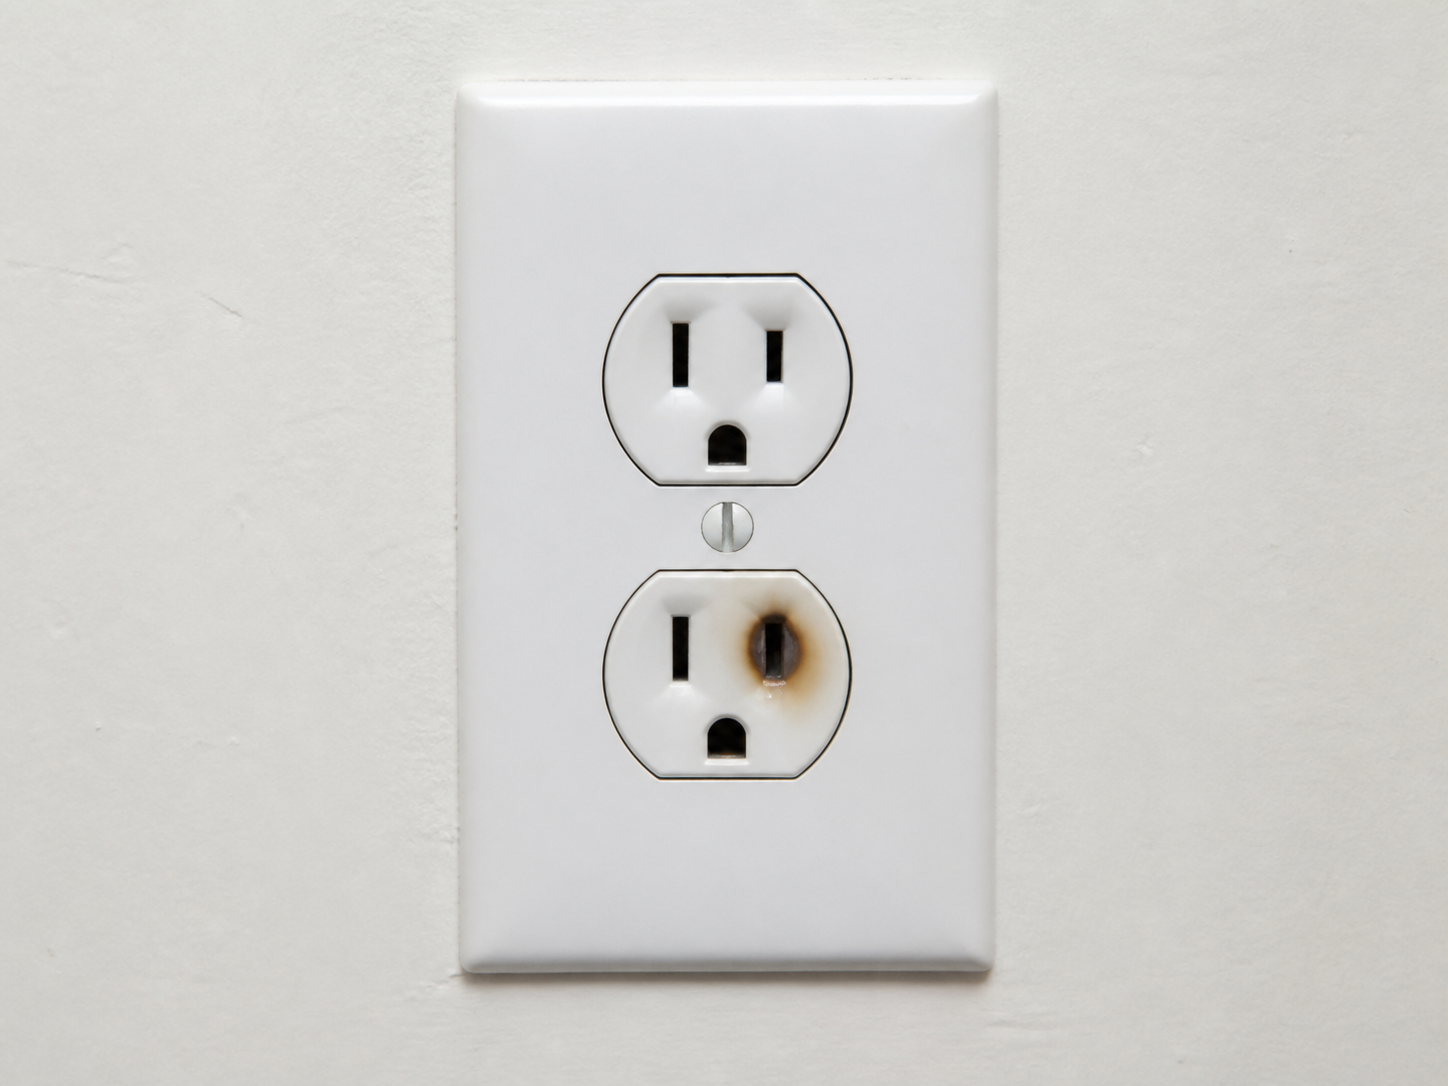
\includegraphics[width=0.45\linewidth]{images/book1/ai/g7-short-circuit-scorched.png}

{\small What a fault leaves behind: overheated current scorched this socket. This is the danger the \omterm{def:g7:short-circuits-safety:fuse}{fuse} and the breaker exist to stop.}
\end{omfigure}

\section{The bodyguards}

\begin{definition}[Fuse]\label{def:g7:short-circuits-safety:fuse}
A \emph{fuse}\index{fuse} is a bodyguard that dies for you: a
deliberately thin wire, \omterm{def:g4:series-circuits:series}{in series} with the circuit it guards,
chosen to \omterm{def:g2:ice-water-steam:meltfreeze}{melt} --- and so cut the loop --- when the current
exceeds its rating. The stampede that would char \omterm{def:g2:measuring-length:units}{metres} of
house wiring instead destroys three \omterm{def:g2:measuring-length:units}{centimetres} of sacrificial
wire in its fireproof cartridge. A blown fuse is replaced ---
\emph{after} the fault is found --- by a fresh one of the same
rating.
\end{definition}

\begin{example}[Breaker and fuse, two guards one duty]\label{ex:g7:short-circuits-safety:breaker}
The modern circuit breaker does the \omterm{def:g7:short-circuits-safety:fuse}{fuse}'s duty without dying: a
spring-loaded \omterm{ex:g3:first-electric-circuit:switch}{switch} that snaps open at the rush and is reset by
a flick --- after the fault is cured. \omterm{def:g7:short-circuits-safety:fuse}{Fuse} or breaker, the
guard's post is the same: \emph{\omterm{def:g4:series-circuits:series}{in series}}, on the \omterm{def:g5:series-parallel-circuits:parallel}{branch} it
protects, so the stampede must pass through its checkpoint. A
guard \omterm{def:g5:series-parallel-circuits:parallel}{in parallel} would watch the rush thunder past on the other
road --- pure decoration.
\end{example}

\begin{example}[Overload: the polite stampede]\label{ex:g7:short-circuits-safety:overload}
Not every dangerous rush is a \omterm{def:g7:short-circuits-safety:device}{short circuit}. A multi-socket
feeding a heater, a kettle and a toaster at once asks its one
\omterm{def:g5:series-parallel-circuits:parallel}{branch} to carry three full marches together --- each appliance
innocent, their sum an overload that warms the wall wiring like
a slow toaster. The breaker trips on the sum, and rightly so.
House rule: one hungry heat-making appliance per socket; the
multi-socket is for lamps and chargers, not for a private
kitchen.
\end{example}

\begin{remark}[The forbidden repair]\label{rem:g7:short-circuits-safety:nail}
The old story is true and still kills: a household's \omterm{def:g7:short-circuits-safety:fuse}{fuse} keeps
blowing, and someone ``repairs'' it with a nail or a coin ---
a stout \omterm{def:g4:conductors-insulators:conductor}{conductor} that will never \omterm{def:g2:ice-water-steam:meltfreeze}{melt}. The symptom is silenced;
the disease rages on. The next stampede meets no checkpoint, and
the house's own wires become the \omterm{def:g7:short-circuits-safety:fuse}{fuse} --- inside the walls.
Never bypass a guard: a \omterm{def:g7:short-circuits-safety:fuse}{fuse} that keeps blowing is a guard that
keeps telling the truth.
\end{remark}

\begin{remark}[The rules, final form]\label{rem:g7:short-circuits-safety:rules}
The family's electrical law-book, with its reasons now complete:
never bridge a \omterm{def:g7:short-circuits-safety:battery}{battery's} \omterm{def:g3:first-electric-circuit:battery}{terminals}, and keep spanners off car
batteries (a \omterm{def:g3:first-electric-circuit:battery}{battery} short in metal is a welding arc); one
heat-hungry appliance per socket (overload); damaged cords
retired (a fraying sleeve is a \omterm{def:g7:short-circuits-safety:device}{short circuit} rehearsing); water
and mains apart, dry hands always (your body must never be the
bypass); guards respected --- matching \omterm{def:g7:short-circuits-safety:fuse}{fuses} only, faults found
before resetting; and the socket itself, forever, not for
fingers or experiments.
\end{remark}

\section{Exercises}

\begin{exercise}[$\star$]\label{exo:g7:short-circuits-safety:1}
State the effortless-road proposition. Why does a bare wire win
the march away from a lamp?
\end{exercise}

\begin{exercise}[$\star$]\label{exo:g7:short-circuits-safety:2}
Distinguish the \omterm{def:g7:short-circuits-safety:device}{short circuit} of a device from the \omterm{def:g7:short-circuits-safety:device}{short circuit}
of the \omterm{def:g3:first-electric-circuit:battery}{battery}. Which is the graver, and why?
\end{exercise}

\begin{exercise}[$\star$]\label{exo:g7:short-circuits-safety:3}
In the safe demonstration, why does \omterm{def:g3:first-electric-circuit:bulb}{bulb} 2 die --- and why does
\omterm{def:g3:first-electric-circuit:bulb}{bulb} 1 brighten at the same moment?
\end{exercise}

\begin{exercise}[$\star$]\label{exo:g7:short-circuits-safety:4}
Why does a \omterm{def:g7:short-circuits-safety:device}{short circuit} \omterm{def:g5:heat-and-insulation:heat}{heat} its wire? What everyday device
uses the same warming on purpose?
\end{exercise}

\begin{exercise}[$\star$]\label{exo:g7:short-circuits-safety:5}
What is a \omterm{def:g7:short-circuits-safety:fuse}{fuse}, and what does it sacrifice? Why must it sit \omterm{def:g4:series-circuits:series}{in
series} with what it guards?
\end{exercise}

\begin{exercise}[$\star$]\label{exo:g7:short-circuits-safety:6}
How does a circuit breaker improve on the \omterm{def:g7:short-circuits-safety:fuse}{fuse}? What must happen
before either guard is reset or replaced?
\end{exercise}

\begin{exercise}[$\star$]\label{exo:g7:short-circuits-safety:7}
A heater, kettle and toaster share one multi-socket. No wire is
bare, no device faulty --- yet the breaker trips. Name the event
and explain the \omterm{def:g5:series-parallel-circuits:parallel}{branch}'s complaint.
\end{exercise}

\begin{exercise}[$\star$]\label{exo:g7:short-circuits-safety:8}
Why is ``repairing'' a \omterm{def:g7:short-circuits-safety:fuse}{fuse} with a nail among the most dangerous
acts in a house? What becomes the \omterm{def:g7:short-circuits-safety:fuse}{fuse} afterward?
\end{exercise}

\begin{exercise}[$\star\star$]\label{exo:g7:short-circuits-safety:9}
A cord's two inner wires, their sleeves frayed, touch each other
inside the cable --- upstream of the lamp they feed. Diagnose:
which kind of \omterm{def:g7:short-circuits-safety:device}{short circuit}, what happens to the lamp, and what
does the \omterm{def:g5:series-parallel-circuits:parallel}{branch}'s guard do?
\end{exercise}

\begin{exercise}[$\star\star$]\label{exo:g7:short-circuits-safety:10}
In the \omterm{def:g3:first-electric-circuit:bulb}{two-bulb} demonstration, predict what happens if the
bypass wire is instead laid across \emph{both} \omterm{def:g3:first-electric-circuit:bulb}{bulbs} together
--- from before \omterm{def:g3:first-electric-circuit:bulb}{bulb} 1 to after \omterm{def:g3:first-electric-circuit:bulb}{bulb} 2. Which definition now
applies, and why must the experimenter not try it?
\end{exercise}

\begin{exercise}[$\star\star$]\label{exo:g7:short-circuits-safety:11}
Christmas morning mystery: grandmother's string of series
\omterm{def:g1:light-and-shadows:source}{fairy-lights} has one \omterm{def:g3:first-electric-circuit:bulb}{bulb} whose inner support wires have fused
together in dying --- short-circuiting itself. Contrary to the
usual tragedy, the \emph{rest of the string keeps shining}, a
little brighter. Explain --- and say what is now slowly being
prepared for the remaining \omterm{def:g3:first-electric-circuit:bulb}{bulbs}.
\end{exercise}

\begin{exercise}[$\star\star\star$]\label{exo:g7:short-circuits-safety:12}
Design the protection plan of a small workshop: three parallel
\omterm{def:g5:series-parallel-circuits:parallel}{branches} (\omterm{def:g1:light-and-shadows:source}{lights}; power tools; a \omterm{def:g3:first-electric-circuit:battery}{battery} charger), one supply.
Place guards and \omterm{ex:g3:first-electric-circuit:switch}{switches}; choose which \omterm{def:g5:series-parallel-circuits:parallel}{branches} deserve their
own guard and why; and write the two-line notice above the \omterm{def:g7:short-circuits-safety:fuse}{fuse}
drawer that summarizes
\cref{rem:g7:short-circuits-safety:nail}.
\end{exercise}

\section{Problem: The Fire Investigator's Report}

\begin{problem}[{Weekend problem --- after the apartment fire; the
investigator reads the wiring's confession; three faults, one
lesson}]\label{pb:g7:short-circuits-safety:1}
Nobody was hurt --- the family was away --- but the kitchen wall
is charred, and the investigator must reconstruct the night from
the evidence. You carry her notebook.

\medskip\noindent\textbf{Part I --- Reading the ruins.}
\begin{enumerate}
  \item Exhibit one: a multi-socket that fed a heater, a kettle
        and a deep-fryer, its plastic half-melted. No bare wires
        anywhere in it. Name the fault this exhibit suggests,
        and why no ``villainous wire'' is needed for it.
  \item Exhibit two: a cord behind the cupboard, chewed by a
        pet, its two \omterm{def:g4:conductors-insulators:conductor}{conductors} touching at the bite. Name this
        fault, and state where the march went from the moment of
        contact.
  \item Exhibit three, the damning one: in the \omterm{def:g7:short-circuits-safety:fuse}{fuse} box, the
        kitchen \omterm{def:g5:series-parallel-circuits:parallel}{branch}'s \omterm{def:g7:short-circuits-safety:fuse}{fuse} cartridge contains --- a rolled
        strip of kitchen foil. State what this ``repair'' did to
        the \omterm{def:g5:series-parallel-circuits:parallel}{branch}'s protection.
  \item Put the three exhibits in a likely story: which fault
        came first, what did the true \omterm{def:g7:short-circuits-safety:fuse}{fuse} do about it (before
        exhibit three), and why did the final night end in fire
        rather than in a dark kitchen?
\end{enumerate}

\medskip\noindent\textbf{Part II --- The physics deposition.}
\begin{enumerate}[resume]
  \item The court asks: why does a shorted or overloaded wire
        \emph{\omterm{def:g5:heat-and-insulation:heat}{heat}}? Give the everyday device that proves
        current-warming can be tamed --- and what was missing
        here.
  \item Why is a \omterm{def:g7:short-circuits-safety:fuse}{fuse} thin on purpose? Explain the phrase ``a
        bodyguard that dies for you''.
  \item The foil strip conducted magnificently. Precisely
        \emph{because} of that, it failed as a guard. Resolve
        the little paradox for the jury.
  \item The heater alone was rated safe, the kettle alone safe,
        the fryer alone safe. Write one sentence on how three
        safeties summed to one danger.
\end{enumerate}

\medskip\noindent\textbf{Part III --- The verdict and the
lessons.}
\begin{enumerate}[resume]
  \item The investigator must rank the three faults by moral
        \omterm{def:g4:weight-and-mass:weight}{weight}: the overload, the chewed cord, the foil. Which
        one turned mishap into catastrophe, and why?
  \item The family asks what would have happened on the fire
        night had a proper \omterm{def:g7:short-circuits-safety:fuse}{fuse} been in place. Walk them
        through it, minute by minute.
  \item Recommend the rewiring: how should heater, kettle and
        fryer be fed now, and what standing rule governs the
        multi-socket's future?
  \item Close the report with the investigator's three-sentence
        summary: the villain's method, the guard's duty, and
        the one repair that must never be improvised.
\end{enumerate}
\end{problem}
